\subsubsection{Melt migration in a 2D mantle convection model}
\label{sec:cookbooks-melt-global}

\textit{This section was contributed by Juliane Dannberg and is based on a section in \cite{dannberg_melt} by Juliane Dannberg and Timo Heister.}

The following cookbook will explain how to use \aspect{}'s implementation of coupled magma/mantle dynamics
(see Section~\ref{sec:melt_transport}) to set up a model of mantle convection that also includes melting
and freezing of mantle rock, and the transport of melt according to the two-phase flow equations.
The model setup is described in detail in \cite{dannberg_melt}, which can be found \href{https://doi.org/10.1093/gji/ggw329}{here},
and in the following we will go over a slightly simplified version in lower resolution.
We will start by looking at a global mantle convection without melt migration, and will
then discuss how the input file has to be modified in order to add melt transport. A movie that compares
the evolution of the temperature field and the amount of melt present in both models in higher resolution can be found
\href{http://youtu.be/Kwyp4Jvx6MU}{online}.

The model setup is a 2D box with dimensions of $2900 \times 8700$\,km, and it is heated from the bottom and
cooled from the top. A full description can be found in Section~4.7 ``Influence of melt migration on a global-scale
convection model'' in \cite{dannberg_melt}.
In the first model we will look at, melting and freezing is only included passively: We use the \texttt{melt fraction} visualization postprocessor to compute how much melt is present for a given temperature and pressure at every given point in time and space in our model, but the presence of melt does not influence material properties like density or viscosity, and melt does not move relative to the solid. This also means that because melt is not extracted, the bulk composition of the material always stays the same, and melt only freezes again once advection or conduction causes the temperature of the solid rock to be below the solidus.
The following input file (which can be found in \url{cookbooks/global_melt/global_no_melt.prm}) contains a detailed description of the
different options required to set up such a model:

\lstinputlisting[language=prmfile]{cookbooks/global_melt/doc/global_no_melt.prm.out}

When we look at visualization output of this model, we can see that over time, first upwellings, and then downwellings start to form. Both are more or less stable over time, and only change their positions slowly. As melt does not move relative to the solid, broad stable zones of melting with melt fraction of 10\% or more form in areas where material is upwelling.

In the second model, melt is an active component of the model. Temperature, pressure and composition control how much of the rock melts, and as soon as that happens, melt can migrate relative to the solid rock. As material only melts partially, that means that the composition of the rock changes when it melts and melt is extracted, and we track this change in composition using a compositional field with the name \texttt{peridotite}. Positive values mark depletion (the composition of the residual host rock as more and more melt is extracted), and negative values mark enrichment (the composition of generated melt, or regions where melt freezes again). Both the fraction of melt (tracked by the compositional field with the name \texttt{porosity}) and the changes in composition influence the material properties such as density and viscosity. Moreover, there are additional material properties that describe how easily melt can move through the host rock, such as the \texttt{permeability}, or properties of the melt itself, such as the \texttt{fluid viscosity}.
The following input file (a complete version of which can be found in \url{cookbooks/global_melt/global_melt.prm}) details the changes we have to make from the first model to set up a model with melt migration:

\lstinputlisting[language=prmfile]{cookbooks/global_melt/doc/global_melt.prm.out}

In the first few tens of millions of years, this models evolves similarly to the model without melt migration. Upwellings rise in the same locations, and regions where material starts to melt are similar. However, once melt is formed, the model evolutions start to deviate. In the model with melt migration, melt moves upwards from the region where it is generated much faster than the flow of solid material, so that it reaches cold regions -- where it freezes again -- in a shorter amount of time. Because of that, the overall amount of melt is smaller in this model at any given point in time. In addition, enriched material, present in places where melt has crystallized, has a higher density than average or depleted mantle material. This means that in regions above stable upwellings, instabilities of dense, enriched material start to form, which leads to small-scale downwellings. Hence, both areas where material is partially molten and the location of the upwellings themselves have a much shorter wavelength and change much faster over time in comparison to the model without melt migration.

\begin{figure}
    \centering
    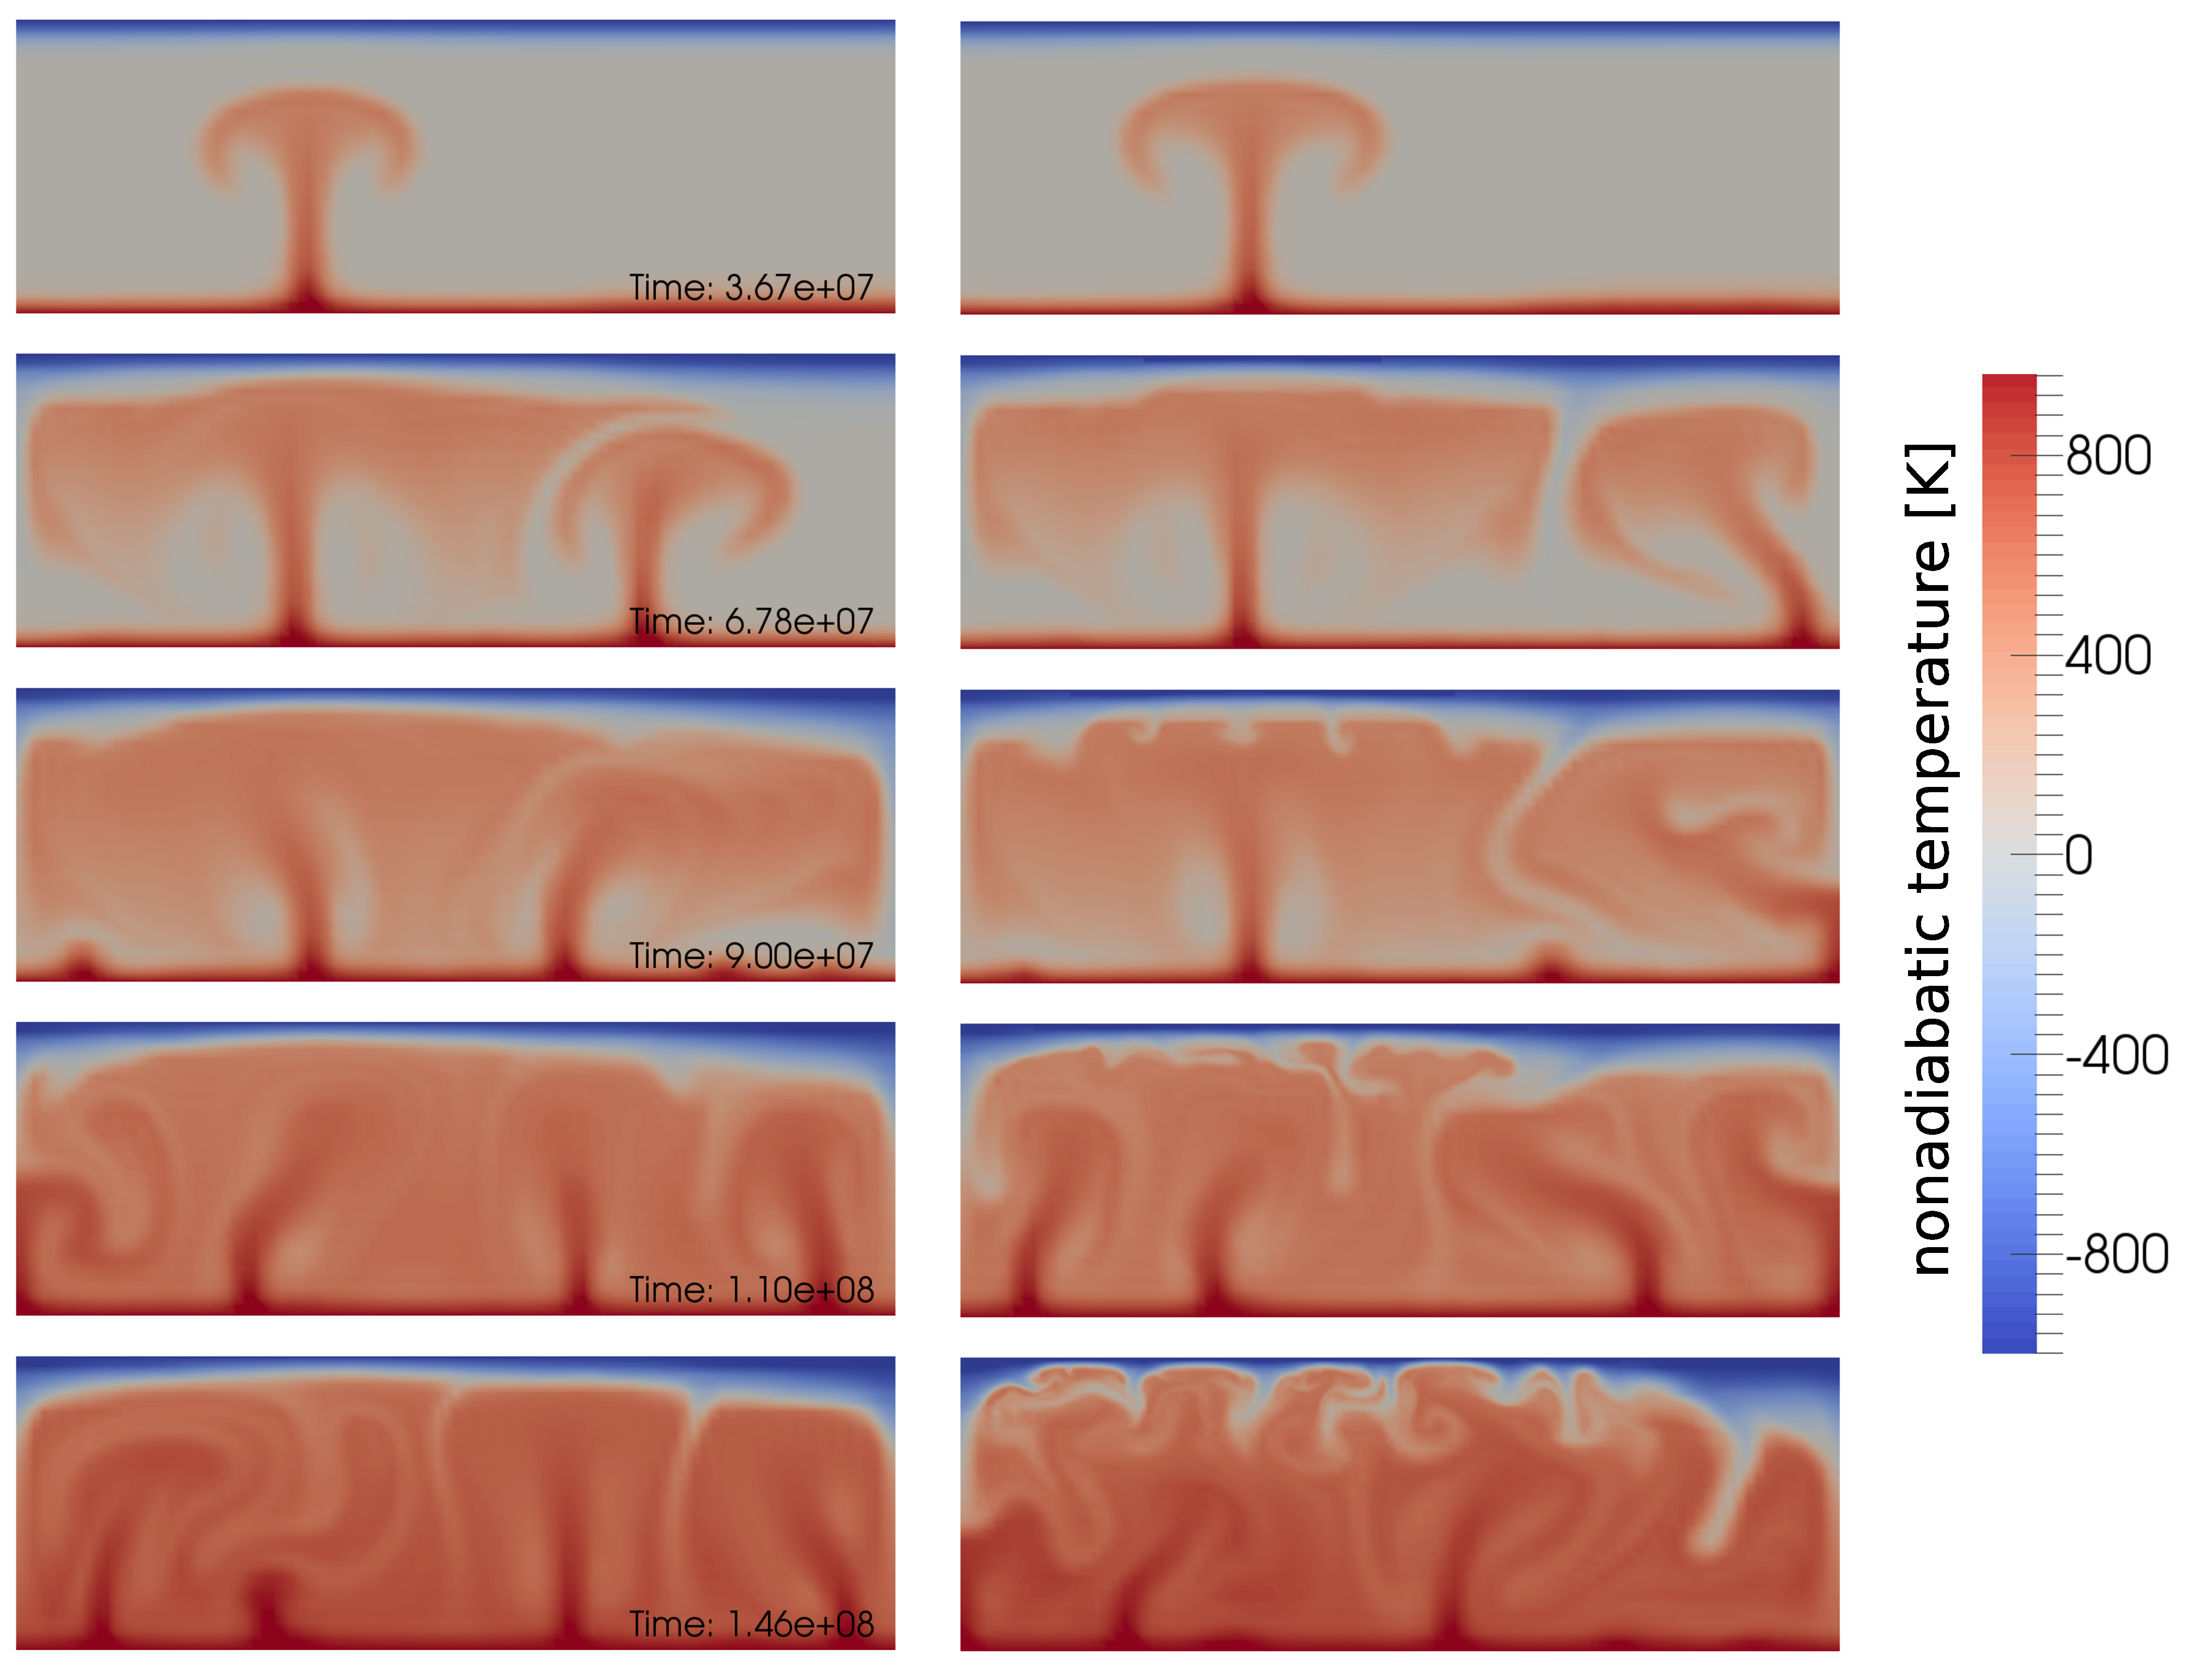
\includegraphics[width=0.9\textwidth]{cookbooks/global_melt/doc/model_evolution.pdf}
    \caption{\it Evolution of the model without (left) and with (right) melt migration.}
    \label{fig:global-melt}
\end{figure}

Figure~\ref{fig:global-melt} shows the time evolution of both models.
A more complete comparison of the two models can be found in Section~4.7 ``Influence of melt migration on a global-scale
convection model'' in \cite{dannberg_melt}.


